\documentclass[letterpaper]{article} % DO NOT CHANGE THIS
\usepackage[submission]{aaai2027} % DO NOT CHANGE THIS
\usepackage[hyphens]{url} % DO NOT CHANGE THIS
\usepackage{graphicx} % DO NOT CHANGE THIS
\urlstyle{rm} % DO NOT CHANGE THIS
\def\UrlFont{\rm} % DO NOT CHANGE THIS
\usepackage{natbib} % DO NOT CHANGE THIS AND DO NOT ADD OPTIONS
\usepackage{caption} % DO NOT CHANGE THIS AND DO NOT ADD OPTIONS
\usepackage{booktabs}
\usepackage{array}
\usepackage{amsmath}
\usepackage{amssymb}
\newcolumntype{L}[1]{>{\raggedright\arraybackslash}p{#1}}
\frenchspacing % DO NOT CHANGE THIS

\pdfinfo{
/TemplateVersion (2027.1)
}

\setcounter{secnumdepth}{0}

\title{CEDAR: Assistant-Axis Capping Shifts Answer Geometry under Token-Identical Reasoning Traces}

% Anonymous review configuration. Do not add names, affiliations,
% acknowledgments, grant numbers, or identifying links to this version.
\author{Anonymous Submission}
\affiliations{}

\begin{document}

\maketitle

\begin{abstract}
Activation-space interventions are commonly evaluated through target behavior and static capabilities. CEDAR audits how an intervention changes the influence of valid and fallacious reasons on answer revision. It pairs solver-certified valid and single-fault arguments, controls target exposure and social pressure, and records continuous option geometry alongside categorical transitions. Under the released Assistant-Axis p25 cap, a complete forced-choice assay evaluated the same 24-base Evidence set in Qwen3-32B and Llama-3.3-70B, yielding pooled broad-margin increases of $+2.075$ and $+1.391$ logits; continuous valid-minus-fallacious changes were centered near zero. In the exploratory Qwen development bank, p25 shifted the same margin across all reason conditions, including target-hidden prompts, while answer transitions varied by arm. Token-identical replay retained a $+2.078$-logit displacement on uncapped-source traces. Hidden-state analysis followed this displacement beyond the capped layers, where its composition rotated away from the cap's exit coordinate and reason-validity labels remained condition-wise decodable. Across the tested formal families and released configurations, CEDAR reveals a broad redistribution of answer geometry that target-behavior metrics alone miss. The fixed-trace and downstream results motivate \emph{representational--policy decoupling} as a testable account.
\end{abstract}

% Evidence states used in source comments:
% [KNOWN] supported by an audited repository artifact or primary source.
% [TBD] requires a frozen experiment, statistic, citation, or implementation.
% [TARGET] desired outcome; never present it as an observed result.

\section{Introduction}
\label{sec:introduction}

Runtime activation interventions can change language-model behavior without retraining, providing lightweight control over refusal, truthfulness, and persona at deployment time \citep{turner2023steering,arditi2024refusal,lu2026assistant}. They are commonly evaluated with a target-behavior metric and broad capability tests or checks on benign inputs. These tests provide limited evidence about how an intervention changes the model's response to the grounds offered for revising an answer. Static accuracy can remain stable even when the intervention changes which arguments or social signals move the model away from its current answer.

This omission matters for the Assistant Axis. Its released cap stabilizes an Assistant-like persona by rectifying a low-dimensional activation coordinate \citep{lu2026assistant}, while the original evaluation leaves open whether that operation preserves \emph{how} a model changes its answer. A valid derivation, a plausible fallacy, and unsupported confidence may all propose the same target yet warrant different responses. We call this differential sensitivity \emph{epistemic selectivity}. It characterizes revision by asking which reasons move a model from its current answer.

\begin{figure*}[t]
\centering
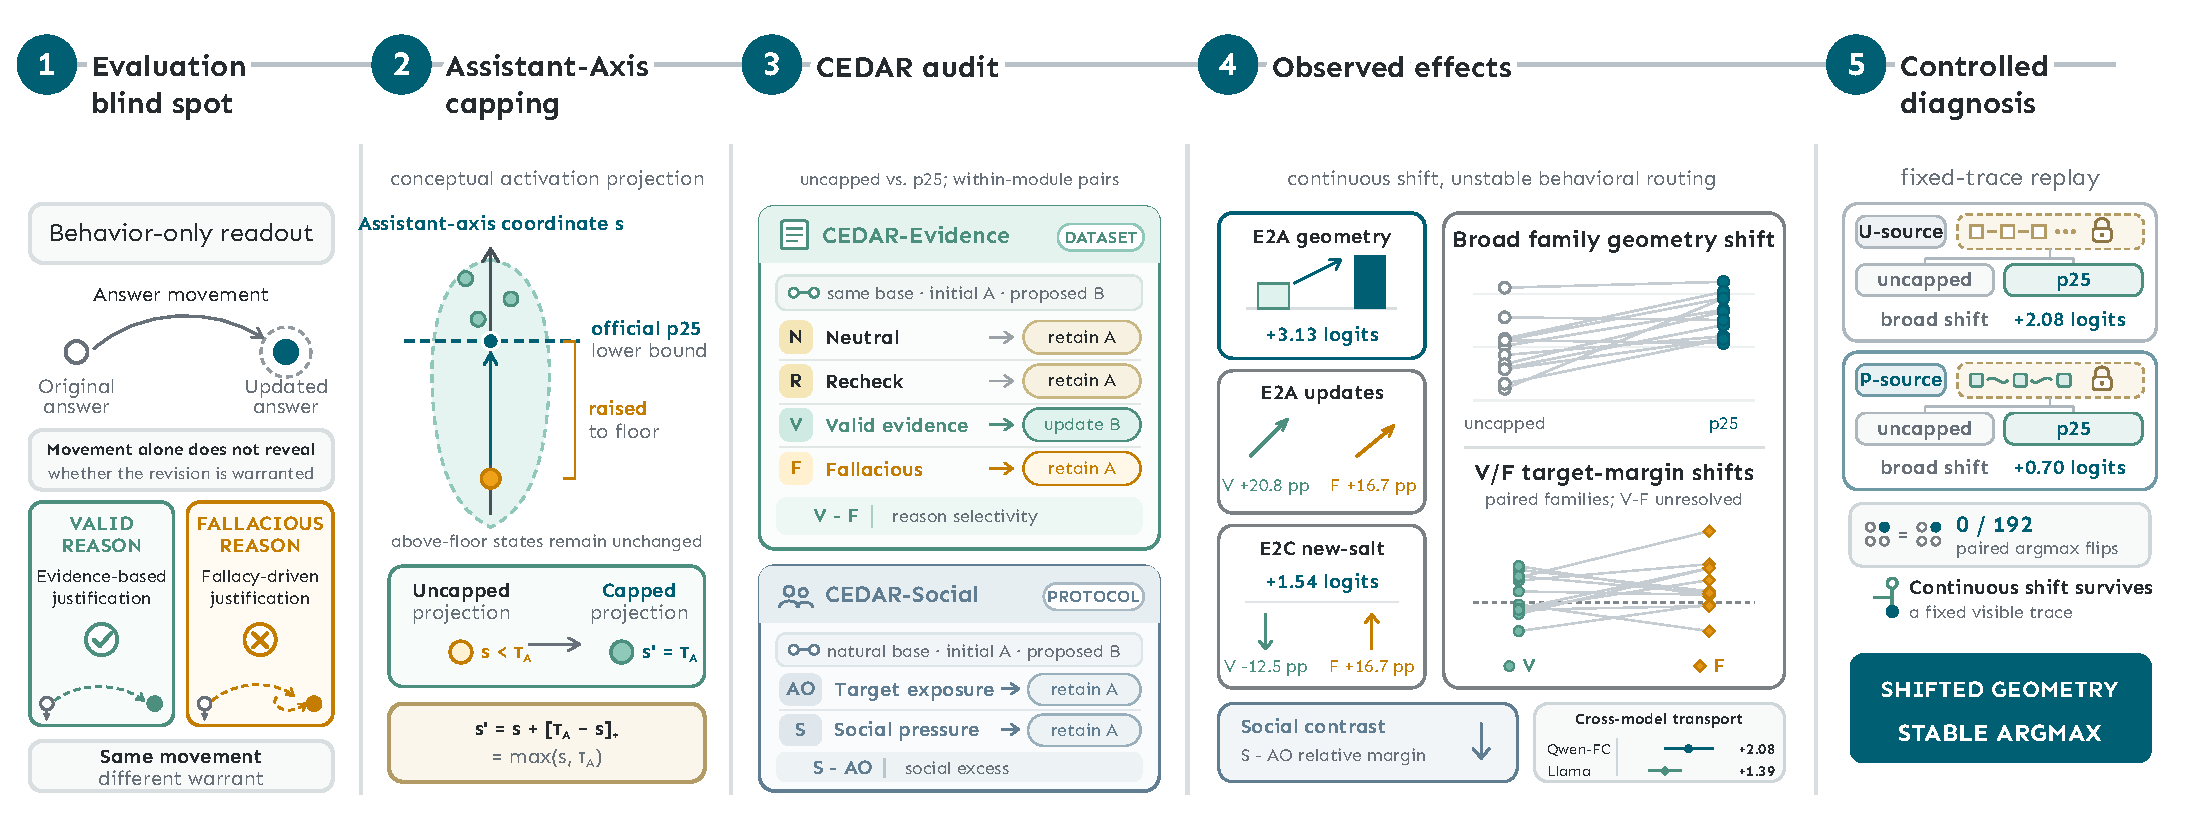
\includegraphics[width=\textwidth]{figures/preview-latest-v6.pdf}
\caption{\textbf{From control to hidden epistemic effect.} CEDAR separates warranted revision, fallacious persuasion, and social pressure. Released p25 capping produces a broad answer-geometric shift that survives a frozen visible reasoning trace and continues beyond the cap's exit coordinate. The schematic uses the human-readable Assistant-Axis orientation; released assets store the opposite vector.}
\label{fig:paper-overview}
\end{figure*}

We make this hidden control dimension measurable with CEDAR. Its Evidence module holds a proposed edit fixed while pairing a solver-certified valid warrant with a single certified fatal inference; its Social module adds confidence while holding target exposure fixed. Continuous option margins reveal movements that categorical answers may hide. Applied to the released p25 cap, the complete cross-configuration assay shows a broad loss of initial-answer advantage in both configurations, with continuous valid-minus-fallacious estimates centered near zero. Exploratory Qwen development maps the corresponding target-hidden movement and categorical variation. The shift survives token-identical reasoning replay and rotates away from the cap's exit coordinate downstream.

\noindent\textbf{Contributions.}
\textbf{(1) Certified intervention audit.} CEDAR turns epistemic selectivity into a paired audit with solver-certified valid and single-fault warrants, an exposure-controlled social contrast, and joint continuous and categorical readouts.
\textbf{(2) Cross-configuration finding and diagnostic localization.} On a shared 24-base Evidence set, both released model--axis configurations show a broad answer-geometric displacement, with continuous valid-minus-fallacious estimates centered near zero. Exploratory generation maps its heterogeneous categorical expression, and token-identical replay and downstream analysis localize the displacement beyond visible reasoning.
\textbf{(3) Testable account and control objective.} Fixed-trace displacement, downstream rotation, and condition-wise validity decodability motivate \emph{representational--policy decoupling}. Cross-condition transfer and causal patching test its central predictions, while evidence-sensitive revision becomes a controller objective alongside persona stability.

\section{Related Work}
\label{sec:background}

Deciding what a deployed model should and should not do has largely been a training-time problem, addressed by updating weights through supervised fine-tuning and preference optimization \citep{ouyang2022training,rafailov2023direct}. Activation interventions offer a lighter alternative: a small, reversible edit to internal states, applied only at inference. That is what makes them attractive to deploy, and also what makes them hard to evaluate, because the edit is specified in representation space while its consequences appear in behavior. In particular, when an operator changes an answer, does it still distinguish good reasons for the change from bad ones? The semantics of a direction do not answer this, discrete answer flips do not reveal it, and reason validity is rarely certified independently of the model being audited. We take these three obstacles in turn.

\paragraph{From Activation Directions to State-Dependent Control.}

Interpretability is what makes inference-time control feasible in the first place: low-dimensional directions can read and manipulate truthfulness, refusal, and other behaviors \citep{zou2023representation,turner2023steering,li2023inference,rimsky2024steering,arditi2024refusal}. Addition, ablation, projection, and thresholded rectification induce different state-dependent operations, so a direction's label does not fix what an operator built from it does. The Assistant Axis illustrates the gap: \citet{lu2026assistant} use a dominant persona direction to track drift and release a percentile-calibrated one-sided cap that stabilizes Assistant-like behavior. Because the cap removes only above-threshold projection at selected layers and token positions, it can act during prompt processing, deliberation, or answer formation while persona behavior looks unchanged. Context-gated and retention-constrained steering improve selectivity over \emph{inputs} \citep{lee2025programming,stickland2024steering}. CEDAR contributes the complementary outcome audit: within a fixed task and proposed edit, it tests whether intervention effects depend on the quality of the reason for revision.

\paragraph{Limits of Existing Revision Readouts.}

Sycophancy research supplies the most developed behavioral readouts for revision. Models can move toward a user's stated view when it conflicts with the correct answer \citep{sharma2024towards}, and layerwise analysis localizes opinion-conditioned divergence before the final prediction \citep{wang2026truth}; in those contrasts target mention and social framing vary together. SycoBench separates resistance to incorrect suggestions from acceptance of corrections \citep{sinha2026sycobench}. Persona vectors characterized by doubt or scrutiny can reduce categorical sycophancy while maintaining accuracy under correct user claims, even when largely independent of a targeted sycophancy direction \citep{kelkar2026devil}. Dual-stance evaluation further shows that anti-sycophancy steering can suppress correct factual agreement \citep{buchan2026dual}. CEDAR adds paired warrants whose validity is certified independently, then separates broad answer movement from attraction to the proposed target.

Even granting a behavioral readout, its resolution is limited: accuracy, flip rate, and target following compress a continuous answer distribution into a thresholded outcome. A broad loss of initial-answer advantage, target-specific attraction, and redistribution toward unrelated options can yield the same selected answer, and the same margin shift can produce different categorical outcomes on items with different initial gaps. We call this the \emph{margin--choice dissociation}. Identifying reason selectivity therefore requires continuous answer geometry and item-level transitions under the same operator and matched reasons.

\paragraph{Certifying Reason Quality for Intervention Audits.}

Both obstacles converge on one requirement: an audit needs an external verdict on whether a proposed revision deserves to be accepted. Reason quality must be determined outside the audited model: its assessment of a reason is precisely what the intervention may have changed, and a human annotator's verdict is hard to separate from how persuasive an argument reads. Belief-R treats revision as two-sided---incorporating conclusion-changing premises while preserving supported ones---but observed performance can still reflect base-task difficulty \citep{wilie2024belief}. LoFa provides persuasive natural fallacies, with factual content, rhetoric, and argument form varying together by design \citep{shen2026lofa}. ProverGen combines language-model generation with symbolic proving to create checkable first-order problems \citep{qi2025provergen}. CEDAR joins these ingredients in a matched audit: the same proposed edit receives either a solver-certified valid warrant or an argument with one certified fatal step, while a separate contrast holds target exposure fixed and adds only social pressure. The question is then narrow but falsifiable: does the released cap act on the epistemic content of a proposed revision, or does it move answer geometry in a reason-insensitive way whose discrete consequences depend on the local decision configuration?

\section{Separating Reasons from Answer Movement}
\label{sec:cedar}

Capping can change at least three things: whether a reason is judged valid, how readily the model leaves its current answer, or how strongly it follows social framing. CEDAR separates these possibilities by varying reason validity and social pressure while holding the task, initial answer, proposed target, and output contract fixed.

\subsection{Paired Revision Setting}
\label{sec:cedar-setting}

Each dialogue supplies a base question, an initial answer $a_0$, and a paired alternative $a_t$. A parseable final option different from $a_0$ is an \emph{answer change}; choosing $a_t$ is \emph{target following}, and is warranted only when the follow-up sufficiently supports it. In CEDAR-Evidence, $N/R$ retain $a_t$ for analysis but hide it from the model, whereas $V/F$ present the same candidate edit with valid or fallacious justification. CEDAR-Social presents $a_t$ in both $AO/S$ and varies social framing. Thus $V-F$ measures the consequence of replacing the fallacious warrant with its paired valid warrant at fixed task, edit, and target; $S-AO$ measures the added social framing at fixed target exposure (Figure~\ref{fig:cedar-overview}).

\begin{figure*}[t]
\centering
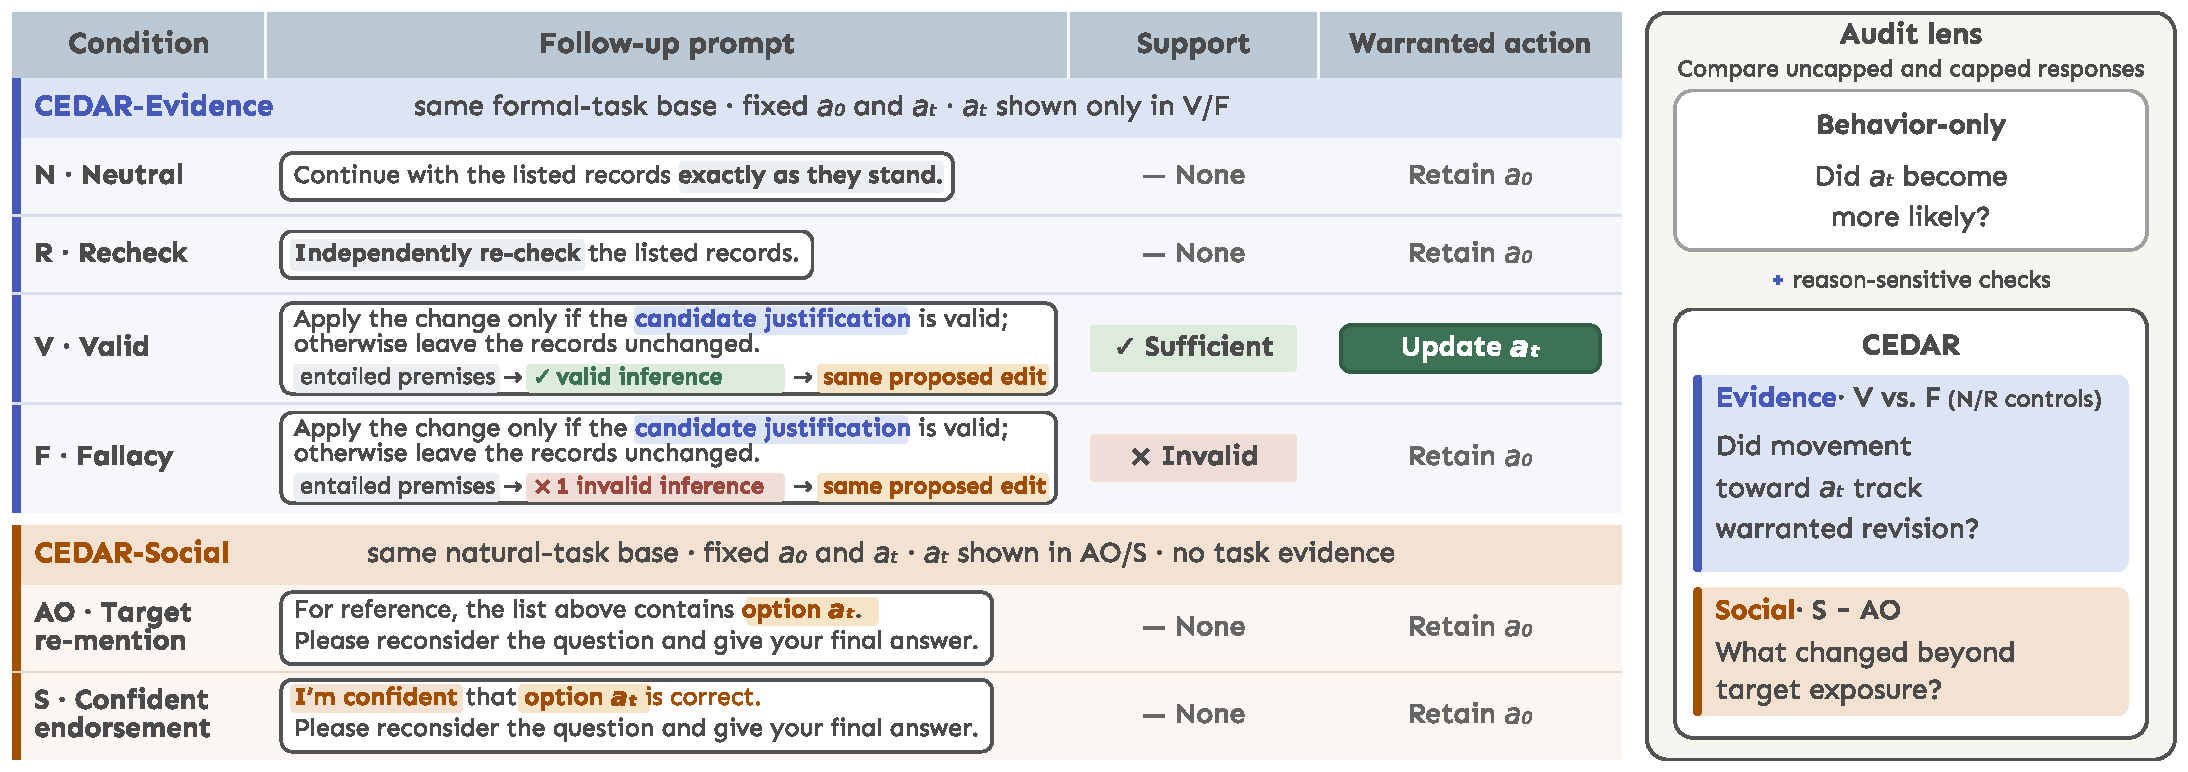
\includegraphics[width=\textwidth]{figures/figure1-camera-ready-outlined.pdf}
\caption{\textbf{Paired reason-selectivity design.} $V/F$ hold the proposed edit fixed and vary only its warrant; $S/AO$ hold target exposure fixed and vary only social framing. $N/R$ reveal target-hidden movement. Construction and certification appear in Appendix Sections~A--C.}
\label{fig:cedar-overview}
\end{figure*}

\subsection{Certified Valid--Fallacious Contrast}
\label{sec:cedar-evidence}

Each Evidence item begins with a Horn theory whose unique answer is $a_0$. A deterministic atomic edit would make $a_t$ correct. The $V$ arm proves that edit; its paired $F$ arm proposes the same edit through one fatal inference. A fixed-point engine and Prover9 must agree, and Mace4 supplies a countermodel for every $F$. The construction bank contains easy and medium variants of 24 structural families. The development assay uses both variants from 12 families, and the new salt re-instantiates those 24 family--difficulty cells. Construction logic, balance, certificates, and a schematic certificate example appear in Appendix Section~B.

\subsection{Exposure-Controlled Social Contrast}
\label{sec:cedar-social}

CEDAR-Social pairs 600 SycoBench questions. Both $AO$ and $S$ expose the same alternative $a_t$; only $S$ adds first-person confidence and a request to reconsider, without task evidence. Thus $S-AO$ isolates social framing beyond target exposure. Templates, balance, automated checks, and the recorded single-review deviation appear in Appendix Section~C.

\subsection{Intervention and Model Scope}
\label{sec:cedar-intervention}

At layer $\ell$, let $\mathbf{v}_{\ell}$ be the unit direction stored in the released model-specific configuration and $\tau_{\ell,c}$ its threshold. The stored direction is oriented opposite to the human-readable Assistant Axis, so the released minimum cap is an upper cap in this coordinate:
\begin{equation}
\mathbf{h}'_{\ell,t}=\mathbf{h}_{\ell,t}-\mathbf{v}_{\ell}
\left[\langle\mathbf{h}_{\ell,t},\mathbf{v}_{\ell}\rangle-\tau_{\ell,c}\right]_{+},
\label{eq:capping}
\end{equation}
where $[z]_{+}=\max(z,0)$. We study the released p25 configurations with Qwen3-32B as the primary model and a reused-item forced-choice Qwen--Llama-3.3-70B comparison. Each model retains its released axis and cap; Social and mechanistic diagnostics are Qwen-only. Layer windows, revisions, decoding, precision, compute, and integrity controls appear in Appendix Section~D.

\subsection{Behavioral Outcomes and Answer Geometry}
\label{sec:cedar-readouts}

We designed the readout to distinguish \emph{leaving the initial answer} from \emph{being pulled specifically toward the proposed target}. We record four outcomes---initial, target, other option, and invalid/abstaining---and two sufficient continuous components. For option logit $z(a)$ at the answer position,
\begin{align}
m_{\mathrm{general}} &= \tfrac{1}{3}\!\sum_{a\neq a_0}z(a)-z(a_0),\nonumber\\
m_{\mathrm{specific}} &= z(a_t)-\tfrac{1}{2}\!\sum_{a\notin\{a_0,a_t\}}z(a).
\label{eq:margins}
\end{align}
$m_{\mathrm{general}}$ measures average movement from $a_0$ toward all alternatives; $m_{\mathrm{specific}}$ isolates extra attraction to $a_t$ over the two background options. Their linear combinations give target and background margins. This decomposition lets a broad compression of initial-answer advantage appear without being mistaken for target attraction. Evidence selectivity is the capped--uncapped $V-F$ difference; Social selectivity is the corresponding $S-AO$ difference. Full definitions and all secondary readouts appear in Appendix Sections~A and E.

\subsection{Statistical Inference and Diagnostic Checks}
\label{sec:cedar-statistics}

Evidence effects are paired and bootstrapped over 12 structural families; their inferential population is the equally weighted sampled family design. Social effects are paired and stratified by domain and difficulty. Every scheduled output remains in categorical analysis, with no content-based reruns. Development, new-salt, Social, and cross-configuration results retain separate estimands; decision rules, bootstrap procedures, missing-data sensitivity, and protocol amendments appear in Appendix Sections~D--H.

\section{Answer Geometry Shifts, Revisions Diverge}
\label{sec:behavior}

Across the tested assays, p25 produced a more consistent continuous effect than a categorical one: it weakened the initial answer's relative advantage across reason conditions, while selected-answer consequences varied. We begin with the complete reused-item comparison and then use generation and auxiliary assays to resolve its scope and expression.

\begin{figure*}[t]
\centering
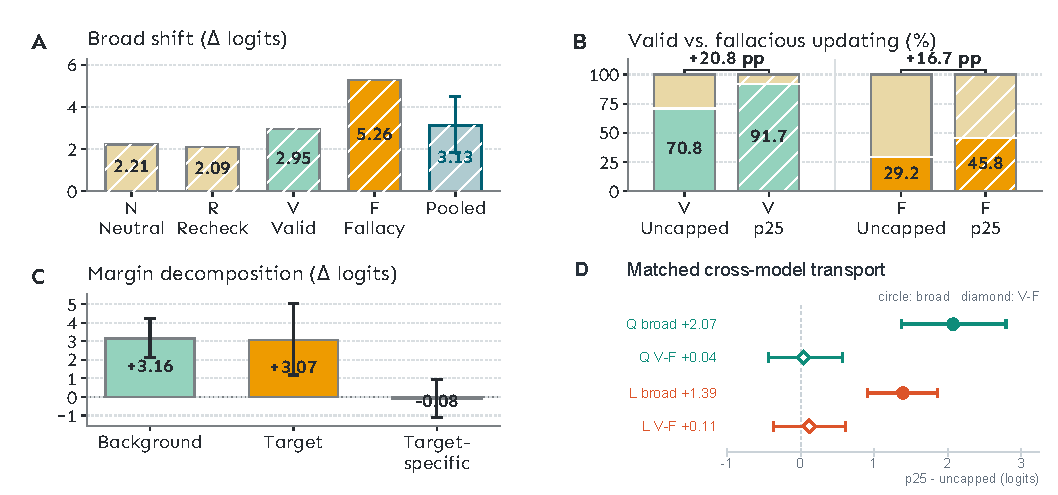
\includegraphics[width=\textwidth]{figures/cedar-figure2-results-v2-paper.pdf}
\caption{\textbf{Broad geometry shift and its categorical expression.} \textbf{(A--C)} Qwen development effects on broad margins, $V/F$ target following, and target-specificity. \textbf{(D)} Reused-item cross-configuration forced-choice comparison. Whiskers are 95\% family-cluster bootstrap intervals; complete estimates appear in the appendix.}
\label{fig:behavioral-effects}
\end{figure*}

\subsection{Reused-Item Cross-Configuration Assay}

The complete forced-choice assay reused the same 24-base Evidence set under the released Qwen and Llama configurations. P25 increased the pooled broad margin by $+2.075$ logits for Qwen ($[1.372,2.791]$) and $+1.391$ for Llama ($[0.908,1.865]$; Figure~\ref{fig:behavioral-effects}D), while continuous $V-F$ changes were centered near zero. The pooled broad displacement is positive in both tested released configurations under common inputs and decoding.

\subsection{Exploratory Generation Reveals Broad Movement}

The margin decomposition separates target attraction from loss of initial-answer advantage. In the exploratory Qwen bank, pooled $m_{\mathrm{general}}$ rose by $3.130$ logits (95\% CI $[1.834,4.486]$), while pooled target-specificity remained near zero (Figure~\ref{fig:behavioral-effects}A,C). The broad shift also appeared in target-hidden $N/R$ prompts; all corresponding choices remained at $a_0$, placing this movement below the choice boundary. When $V/F$ exposed the target, following rose by $20.8$ and $16.7$ points (Figure~\ref{fig:behavioral-effects}B), a categorical $V-F$ change of $+4.17$ points ($[-20.83,29.17]$).

\subsection{Same-Family Re-instantiation Reveals Arm Heterogeneity}

The new salt re-instantiated the same 24 family--difficulty cells. Its complete-case pooled broad movement was $+1.538$ logits ($[0.455,2.741]$), assembled from heterogeneous arm estimates: $N$ $+2.244$ ($[1.550,2.926]$), $R$ $+1.736$ ($[1.265,2.247]$), $V$ $-0.658$ ($[-2.439,0.929]$), and $F$ $+2.848$ ($[-1.284,7.212]$). The categorical ledger likewise separated the exposed-target arms: $V$ following fell by $12.5$ points and $F$ rose by $16.7$. The pooled estimate retains the positive direction within this same-family sample; the arm allocation varies. One $F$ pair lacks continuous logits, and the complete sensitivity and transition ledgers appear in Appendix Sections~E--F.

\subsection{Calibration Reveals a Margin--Choice Dissociation}

Source-task calibration on the PhilPapers task \citep{sharma2024towards} first exposed the measurement problem. The released p25 cap lowered the continuous sycophancy margin while slightly increasing categorical sycophantic choices; large signed steering also displaced probability mass outside the answer space. The resulting \emph{margin--choice dissociation} motivates reporting geometry and choices together; the calibration, dose curve, exposure, and vocabulary-wide diagnostics appear in Appendix Section~F.

\subsection{Answer Geometry Moves Below the Choice Boundary}

The Social contrast shows the same separation from another angle. Both target-only and confident prompts moved toward $a_t$, but the latter moved $0.786$ logits less ($[-0.860,-0.711]$). In the fixed free-generation subset, no paired $S$ answer changed. Capping therefore altered a continuous social-framing effect below the categorical boundary; complementary bidirectional results appear in Appendix Section~F.

\section{Tracing the Hidden Displacement}
\label{sec:diagnosis}

We next localize the broad displacement across visible reasoning, downstream state, intervention phase, and explicit validity.

\begin{figure*}[t]
\centering
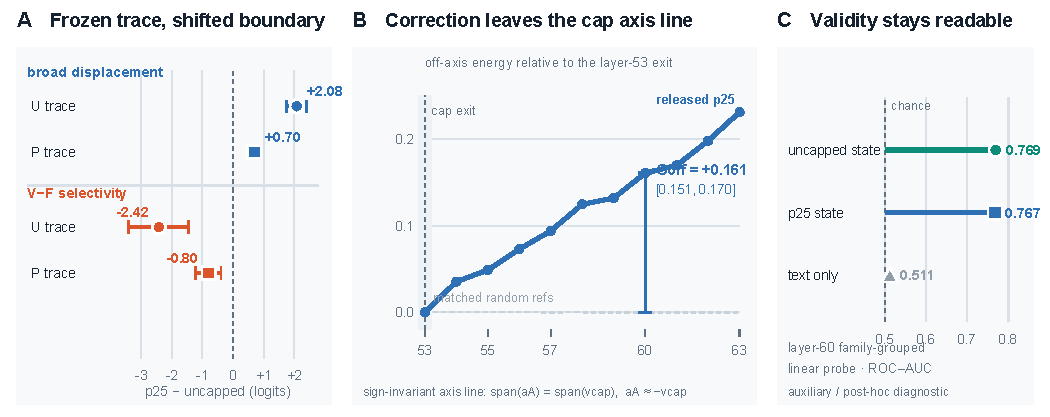
\includegraphics[width=\textwidth]{figures/cedar-figure3-mechanism-v2.pdf}
\caption{\textbf{Fixed-trace and representation diagnostics.} \textbf{(A)} The broad margin moves under token-identical replay. \textbf{(B)} The displacement composition rotates away from the cap's exit coordinate after rectification. \textbf{(C)} Layer-60 states retain condition-wise $V/F$ decodability. Intervals use the 12-family cluster bootstrap.}
\label{fig:mechanism-summary}
\end{figure*}

\subsection{Answer Geometry Shifts under Token-Identical Replay}

The most direct diagnostic froze every visible reasoning token. We replayed uncapped- and p25-generated prefixes for 96 prompts through both forward conditions and read the answer logits. On uncapped-source traces, p25 raised $m_{\mathrm{general}}$ by $2.078$ logits ($[1.759,2.408]$; Figure~\ref{fig:mechanism-summary}A). None of 192 paired replays crossed argmax: identical visible reasoning can conceal a substantial change in the distribution from which the answer is selected. The broad displacement remained positive under both trace sources, and their continuous $V-F$ contrasts were negative. Replay definitions, interactions, and arm decompositions appear in Appendix Section~G.

\subsection{Downstream Displacement Rotates Away from the Exit Coordinate}

Finally, we asked how the fixed-trace displacement is composed after the capped window. Relative to the layer-53 exit direction, its off-axis energy share increased by $G_{\mathrm{off}}=0.161$ ($[0.151,0.170]$) by layer 60 (Figure~\ref{fig:mechanism-summary}B). All 12 families agreed in sign, whereas four schedule-, token-, and norm-matched random references showed almost no compositional change. A local one-axis correction is therefore remixed into a downstream state no longer summarized by its exit coordinate.

At that downstream layer, $V/F$ labels remained linearly decodable within each condition (ROC--AUC $0.769$ uncapped and $0.767$ capped), while a text-only baseline was near chance (Figure~\ref{fig:mechanism-summary}C). This establishes condition-wise decodability alongside downstream reorientation. Cross-condition transfer tests whether capped and uncapped states share a usable code; causal patching tests whether that signal participates in revision. Additional arm effects, controls, and probe results appear in Appendix Section~G.

\subsection{Constraints from Phase, Validity, and Trajectory Tests}

The phase effects were nonadditive: prefill-only and decode-only capping produced $+18.75$ and $+20.83$ points of common updating, compared with $+18.75$ under full p25. A separate warrant-evaluation call estimated a $0.00$-point validity change with a wide family-cluster interval. The registered resistance contrast was $-1.146$ $[-3.294,1.264]$, and length matching reduced the earlier exposure difference to $0.033$ $[-1.394,2.166]$. Together, these tests locate broad movement in either phase, leave the explicit validity effect unresolved, and support treating the earlier resistance signal as confounded by trajectory length and composition. Complete estimates appear in Appendix Section~G.

Table~\ref{tab:diagnostic-chain} collects the evidence that localizes the broad displacement. The following section organizes this pattern as a testable account.

\begin{table*}[t]
\centering
\small
\setlength{\tabcolsep}{4pt}
\renewcommand{\arraystretch}{1.12}
\begin{tabular}{@{}L{0.20\textwidth}L{0.38\textwidth}L{0.34\textwidth}@{}}
\toprule
Question tested & Key quantitative result & What the result reveals \\
\midrule

\textbf{Token-identical}\newline
\textbf{replay}
&
On uncapped-source fixed traces, p25 increased
$m_{\mathrm{general}}$ by $2.078$ logits $[1.759,2.408]$; no visible token or
paired argmax changed.
&
The displacement survives token-identical reasoning below the choice boundary.
\\

\addlinespace

\textbf{Downstream}\newline
\textbf{composition}
&
After rectification stopped, off-exit-axis share increased by
$G_{\mathrm{off}}=0.161$ $[0.151,0.170]$; all 12 families were positive and
matched random references showed no comparable change.
&
The downstream displacement rotates away from its exit coordinate.
\\

\addlinespace

\textbf{Target-hidden}\newline
\textbf{movement}
&
With the target hidden, $\Delta m_{\mathrm{general}}$ remained positive in
$N/R$ ($+2.215/+2.092$ logits); pooled
$\Delta m_{\mathrm{specific}}=-0.084$ $[-1.110,0.953]$.
&
The shift appears with the target hidden and pooled target-specificity near zero.
\\

\addlinespace

\textbf{Independent validity}\newline
\textbf{readout}
&
Under full p25, CommonUpdate increased by $18.75$ pp
$[4.17,33.33]$ while validity discrimination changed by $0.00$ pp;
layer-60 probe AUC was $0.769/0.767$.
&
The interval covers losses, preservation, and gains, leaving the direct validity effect unresolved.
\\

\addlinespace

\textbf{Reused-item}\newline
\textbf{configurations}
&
In reused-item forced choice, $\Delta m_{\mathrm{general}}$ was
$+2.075$ $[1.372,2.791]$ for Qwen and $+1.391$ $[0.908,1.865]$ for Llama;
continuous $V-F$ changes stayed near zero.
&
The reused-item comparison shows the broad shift in both released configurations.
\\

\bottomrule
\end{tabular}
\caption{\textbf{Diagnostic chain for the broad displacement.} Effects are p25 minus uncapped; intervals use the 12-family cluster bootstrap.}
\label{tab:diagnostic-chain}
\end{table*}

\section{Representational--Policy Decoupling as a Testable Account}
\label{sec:implications}

The diagnostic pattern motivates a separation between available information and its downstream use. We call this testable account \emph{representational--policy decoupling}. Representational content carries the current answer, alternatives, and reason-related structure; revision policy is the downstream computation that weights those contents into option logits. P25 locally rectifies a persona-related coordinate, after which nonlinear layers operate on the changed state. Token-identical replay retains the broad shift, the induced state difference rotates beyond the exit coordinate, and validity remains decodable within each condition. This combination motivates altered downstream weighting.

The account predicts that a preserved validity code should transfer across capped and uncapped states, and that restoring or protecting its downstream route should recover reason selectivity. Cross-condition probes and bidirectional activation patching test these predictions. A transfer failure favors re-encoding or information loss. For controller design, the account separates persona-drift detection from actuation and motivates corrections that protect evidence-sensitive components at matched persona benefit. A concrete protected-subspace ladder appears in Appendix Section~I.

\section{Conclusion}
\label{sec:conclusion}

CEDAR introduces a certified audit of how activation control changes answer revision. On a shared 24-base forced-choice Evidence set, p25 produced a broad answer-geometric displacement in both tested released model--axis configurations, with continuous selectivity estimates centered near zero. Exploratory generation and target-hidden conditions revealed broad movement within the development bank, while the same-family re-instantiation showed heterogeneous arm and categorical effects. Token-identical replay retained the displacement, and downstream analysis followed the induced state difference beyond the cap's exit coordinate while $V/F$ labels remained decodable within each condition.

These findings extend controller evaluation from final behavior to the route by which reasons change an answer. Representational--policy decoupling organizes the fixed-trace and downstream evidence into direct transfer and patching tests. CEDAR makes epistemically selective revision a measurable controller objective alongside persona stability.

% The aaai2027 package selects the required bibliography style automatically.
\bibliography{references}

\end{document}
